\section{A Jordan theorem on the square grid}\label{sec:grid}
A parity familiar from drawing a ray from a point has a second use. It proves that each side of a simple grid polygon is connected, and computes the number of regions even when the drawing has many cycles.

\subsection{A boundary with an explicit inverse}
Use an $a$ by $b$ rectangle of unit squares, with $a,b\ge1$, and include its exterior as one extra face $*$. A primal edge is a unit horizontal or vertical segment. Its two incident faces include $*$ when it is on the frame. A drawing $G$ is any specified subset of primal edges, with specified vertices containing their endpoints. Additional isolated vertices are allowed. For now the word \emph{region} means a component of the dual graph on faces in which we delete exactly the adjacencies across $G$. For a bit $s$ on each face, with $s(*)=0$, define $\partial s(e)$ to be the exclusive-or of the bits of the two faces at $e$.

\begin{lemma}[Filling an even grid chain]\label{lem:gridfill}\label{idx-plane7}
An edge mask $z$ is of the form $\partial s$ exactly when the number of marked edges at every grid vertex is even. The face mask $s$ with exterior bit zero is unique, and one horizontal scan per row computes it.
\end{lemma}
\begin{proof}
Around a vertex the incident faces form a circular list, with exterior sectors filled by $*$. The sum modulo two of successive differences around this list is zero. Conversely, extend $z$ by zero outside the rectangle. Write $v_{i,j}$ for the bit on $(i,j)(i,j+1)$ and $h_{i,j}$ for the bit on $(i,j)(i+1,j)$. For the square with lower left corner $(i,j)$ put
\[
 s_{i,j}=\bigoplus_{u\le i} v_{u,j}.
\]
The sum starts with $u=0$. Its value is zero on the whole far right: the vertex parity equations summed over vertices at heights at most $j$ cancel all internal edges and give $\bigoplus_u v_{u,j}=0$. Values outside the other three sides are also zero. Crossing a vertical edge changes the scan by its bit. At vertex $(u,j)$ the parity equation is
\[
 v_{u,j}\oplus v_{u,j-1}=h_{u,j}\oplus h_{u-1,j}.
\]
Summing over $u\le i$ gives $s_{i,j}\oplus s_{i,j-1}=h_{i,j}$. This verifies every edge, including the frame. Two fillings with the same differences agree by scanning from the exterior along each row.
\end{proof}

\begin{theorem}[Euler's planar region formula]\label{thm:gridEuler}\label{idx-plane22}
For a grid drawing with $V$ vertices, $E$ edges, $c$ primal components and $F$ regions, including the unbounded one,
\[
                  V-E+F=1+c .
\]
The formula includes the empty drawing. Every region has a representative face computable from the drawing.
\end{theorem}
\begin{proof}
Face masks with $s(*)=0$ that are constant on each region are in bijection with $F-1$ free bits. The lemma takes precisely these masks to even subgraphs contained in $G$. To count those, grow a spanning forest by scanning the edges, inserting one when its ends have distinct current components. An insertion merges two components. At termination every original edge has its endpoints in one tree, so exactly $V-c$ edges were inserted. Prescribe arbitrary bits on the $E-V+c$ remaining edges. For a chosen remaining edge with bit one, add it and the unique tree path between its ends modulo two. Their sum over the choices is even and has the prescribed bits. The difference of two solutions is an even subgraph of a forest. A nonempty such subgraph has a leaf, as one sees by taking a longest simple path, contradicting even degree. Thus $2^{F-1}=2^{E-V+c}$ and injectivity of the powers of two gives the result. All paths needed here have length at most $V$ and can be obtained by recording parents in a finite search. Isolated primal vertices each increase both $V$ and $c$ by one.
\end{proof}

\begin{theorem}[Grid Jordan separation, with paths]\label{thm:gridJordan}\label{idx-plane33}
A simple closed lattice edge polygon has exactly two regions. Exactly one is bounded. Every edge of the polygon has one face in each, and any two rational points of its complement in the same region can be joined by an explicitly computable rational polygonal path missing the polygon.
\end{theorem}
\begin{proof}
Pad the surrounding rectangle by at least one layer of squares. The polygon graph has $E=V$ and $c=1$, hence $F=2$. Its full edge mask is even. Its unique filling from Lemma~\ref{lem:gridfill} has opposite bits at every polygon edge and equal bits at all other edges. Both bits occur. Each region has a constant bit, so the bits distinguish the two regions. The exterior bit is zero. The other region consists of finitely many squares, incident free edges, and free vertices within the frame.

For a rational point off the polygon, determine the grid face, open edge, or vertex containing it by exact rational comparisons. If it is on a free edge, the two incident squares communicate. At a free vertex all incident squares communicate around it. A straight segment from the point to a chosen incident square center stays clear. If it lies outside the frame, enlarge the padded rectangle to include the point in its interior. Breadth-first search on adjacent faces of the same bit gives a path of length at most $ab$ between two such squares, routing through the padding instead of $*$ if needed. Indeed the ring of boundary squares is connected and misses the polygon. Join successive centers through the midpoint of their common edge. This constructs the asserted path and shows the entire zero side extends to infinity. An isolated primal vertex in the preceding theorem can likewise be avoided by moving within a tiny punctured square.

For the converse, the bit extends locally constantly to the complement. A small open box about a point off the polygon meets only incident free squares if it is centered sufficiently close to that point. More quantitatively, the bit cannot change along a rational segment missing the polygon: cut the segment at its intersections with grid lines, treating a part on a grid line as an open edge. Each transition crosses a free edge or goes through a free vertex. Thus no polygonal path crosses sides. For a continuously presented path given a clearance $\eta>0$ from the polygon and a uniform modulus, sample it to within $\eta/8$ on a mesh of oscillation $<\eta/8$. Its rational polygonal interpolation misses the polygon and has endpoints on the original sides. This also rules out such a presented crossing. The geometric boundary of both regions is the polygon: each edge has both bits, each polygon vertex is a limit of points on its incident edges, and the bit is locally constant everywhere else.
\end{proof}

\begin{center}
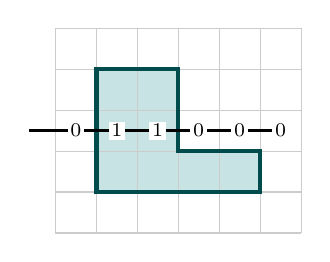
\begin{tikzpicture}[scale=.52]
\fill[teal!22] (1,1)--(5,1)--(5,2)--(3,2)--(3,4)--(1,4)--cycle;
\draw[step=1,gray!40,thin] (0,0) grid (6,5);
\draw[teal!60!black,line width=1.6pt] (1,1)--(5,1)--(5,2)--(3,2)--(3,4)--(1,4)--cycle;
\draw[->,thick] (-.65,2.5)--(5.7,2.5);
\foreach \x/\b in {0.5/0,1.5/1,2.5/1,3.5/0,4.5/0,5.5/0}
  \node[fill=white,inner sep=1pt] at (\x,2.5) {\scriptsize $\b$};
\end{tikzpicture}

{\small The scan toggles at each vertical polygon edge. A horizontal edge is\par
 accounted for by the parity equations in the two adjacent rows.}
\end{center}

\paragraph{Coordinate and arithmetic scope.}
Scaling by a common positive denominator and subdividing proves the same statements for simple rational rectilinear polygons. The number of grid cells can be large in the bit length of the coordinates but is primitive recursive in their numerical codes. The longest searches above may instead enumerate paths of length at most the number of graph vertices, with codes bounded by $(2+ab+a+b)^{2(ab+a+b+3)}$ for the dual walks. The row invariant in Lemma~\ref{lem:gridfill} is an equation of prefix parity bits. The assertion that all forest paths of length at most $V$ have the claimed cancellation is a bounded test. These are permissible induction formulas after Boolean compilation. Arbitrary Jordan embeddings require different separation information.

\begin{corollary}[The circle separates the plane]\label{cor:circlePlane}\label{idx-plane61}
For points equipped with positive distance from the unit circle, its complement in the presented plane has exactly two path components, the inside and the outside. Each point of the circle is in the boundary of both.
\end{corollary}
\begin{proof}
For the square $\|x\|_\infty=1$, a positive gap permits deciding the sign of $\|x\|_\infty-1$ from one sufficiently fine reading. The inside is convex, so contracts by straight segments. For two outside points choose a rational $R$ larger than both norms. Travel out each ray to the boundary of the square of radius $R$ and join the endpoints along that square. The latter path exists constructively by its perimeter parametrization: take a rational lift near each endpoint and interpolate in the covering line (use a radius-$1/4$ local chart to lift each named endpoint). Along the whole route the norm is at least the smaller original norm. No uniformly presented path with positive uniform clearance can join the two signs, since its norm along the path would take values arbitrarily close to $1$ by the approximate intermediate value theorem. The same holds when a pointwise positive clearance with a PR local test for the two signs is supplied, by the local connectedness test in Section~\ref{sec:metric-names}: signs restrict to an extensional locally constant bit on the parameter interval when a sign evaluator is supplied. For each square boundary point $p$, the points $(1\pm 2^{-j})p$, $j\ge1$, approach from the two sides. The explicit radial transformations in Section~\ref{sec:metric-names} are defined on the full plane, carry the square boundary to the unit circle, and carry each of the two strict norm inequalities to the corresponding Euclidean one. Their Lipschitz bounds transport positive clearance, giving the conclusion in the indicated path presentations.
\end{proof}
